\documentclass[journal,onecolumn]{IEEEtran}
\usepackage{graphicx}
\usepackage{booktabs}
\usepackage{multirow}
\usepackage{float}
\usepackage{placeins}
\usepackage{amsmath}
\usepackage{amssymb}

\graphicspath{{./images/}}

\begin{document}

\title{Supplementary Materials for\\
ADMET-Bench: Task-Dependent Performance of GNNs and Pretrained Models in ADMET Prediction}

\author{}

\maketitle

\renewcommand{\thetable}{S\arabic{table}}
\renewcommand{\thefigure}{S\arabic{figure}}

\section{Architecture-Selection Experiments}
\label{sec:supp_architecture}

This section reports the preliminary architecture-selection screen used to choose the graph neural network backbone. Eight message-passing variants (GraphConv, GCN, GAT, GraphSAGE, GIN, TAG, SGC, and TransformerConv) were evaluated on all six benchmark endpoints under the same scaffold-split pipeline, target transformations, and evaluation metrics used in the main study. For each architecture and endpoint the reported result is the best of five configurations selected on the validation split (search over hidden dimension, number of layers, and learning rate), giving $8 \times 6 \times 5 = 240$ training runs in total.

\begin{table}[H]
\centering
\caption{Preliminary classification architecture screen: \emph{validation}-split AUC-ROC and F1 (the model-selection basis), each architecture at its best of five validation-selected configurations. Best validation AUC per task in \textbf{bold}. Test-set performance was not used for architecture selection.}
\label{tab:arch_classification}
\small
\setlength{\tabcolsep}{4pt}
\begin{tabular}{lcccc}
\toprule
\textbf{Architecture} & \multicolumn{2}{c}{\textbf{Tox21 (NR-AR)}} & \multicolumn{2}{c}{\textbf{hERG}} \\
 & \textbf{Val AUC} & \textbf{Val F1} & \textbf{Val AUC} & \textbf{Val F1} \\
\midrule
GraphConv & 0.819 & 0.480 & 0.918 & 0.903 \\
GCN & 0.821 & 0.435 & 0.912 & 0.915 \\
GAT & 0.819 & 0.500 & 0.907 & 0.871 \\
GraphSAGE & \textbf{0.854} & 0.421 & 0.903 & 0.918 \\
GIN & 0.844 & 0.500 & 0.884 & 0.933 \\
TAG & 0.821 & 0.444 & 0.892 & 0.897 \\
SGC & 0.829 & 0.500 & \textbf{0.920} & 0.875 \\
Transformer & 0.778 & 0.480 & 0.905 & 0.881 \\
\bottomrule
\end{tabular}
\end{table}

\begin{table}[H]
\centering
\caption{Regression architecture screen: average rank across the four ADME regression datasets by \emph{validation} R$^2$ (lower rank is better), the basis on which the backbone was selected; each architecture at its best of five validation-selected configurations. Per-dataset validation R$^2$ shown; the final column gives mean \emph{test} R$^2$ as a post-hoc reference only (not used for selection). GraphConv (deployed backbone) in \textbf{bold}.}
\label{tab:arch_regression}
\small
\setlength{\tabcolsep}{4pt}
\begin{tabular}{lcccccccc}
\toprule
\textbf{Arch.} & \textbf{Avg Rank} & \textbf{Caco-2} & \textbf{Half-Life} & \textbf{Clear. Hep.} & \textbf{Clear. Mic.} & \textbf{Test R$^2$} & \textbf{Params} & \textbf{Time (s)} \\
\midrule
GraphSAGE & 3.00 & 0.597 & 0.434 & 0.316 & 0.175 & 0.096 & 662k & 7.3 \\
Transformer & 3.25 & 0.606 & 0.335 & 0.327 & 0.208 & $-$0.197 & 316k & 16.4 \\
TAG & 4.25 & 0.582 & 0.407 & 0.228 & 0.279 & 0.226 & 1059k & 12.2 \\
\textbf{GraphConv} & 4.25 & 0.575 & 0.460 & 0.267 & 0.081 & $-$0.673 & 81k & 7.1 \\
GCN & 4.75 & 0.534 & 0.447 & 0.247 & 0.137 & $-$0.673 & 399k & 12.8 \\
GAT & 5.00 & 0.513 & 0.483 & 0.233 & 0.122 & 0.128 & 1067k & 14.9 \\
SGC & 5.50 & 0.560 & 0.426 & 0.194 & 0.159 & 0.006 & 463k & 12.6 \\
GIN & 6.00 & 0.625 & 0.368 & 0.157 & 0.058 & $-$1.572 & 113k & 6.2 \\
\bottomrule
\end{tabular}
\end{table}

No architecture dominates. Ranked by \emph{validation} performance (the only leak-free selection signal), the eight backbones span a narrow average regression rank ($3.0$--$6.0$) with small per-dataset differences, and every architecture is unstable, with several collapsing to large negative test R$^2$, on the weakly-learnable clearance and half-life endpoints. This validation ordering is a poor predictor of test performance: the best validation-ranked backbone (GraphSAGE) reaches only mean test R$^2 = 0.10$, while several validation-competitive backbones post negative mean test R$^2$ (down to $-1.57$). GraphConv is mid-ranked on validation (regression validation rank $4.25$ of $8$) and is not a test-maximizing choice (its mean test R$^2$ is among the lowest); it was adopted as a single representative backbone, and because architecture selection used validation metrics only, the main-benchmark test evaluation remains unbiased.

\begin{figure}[H]
    \centering
    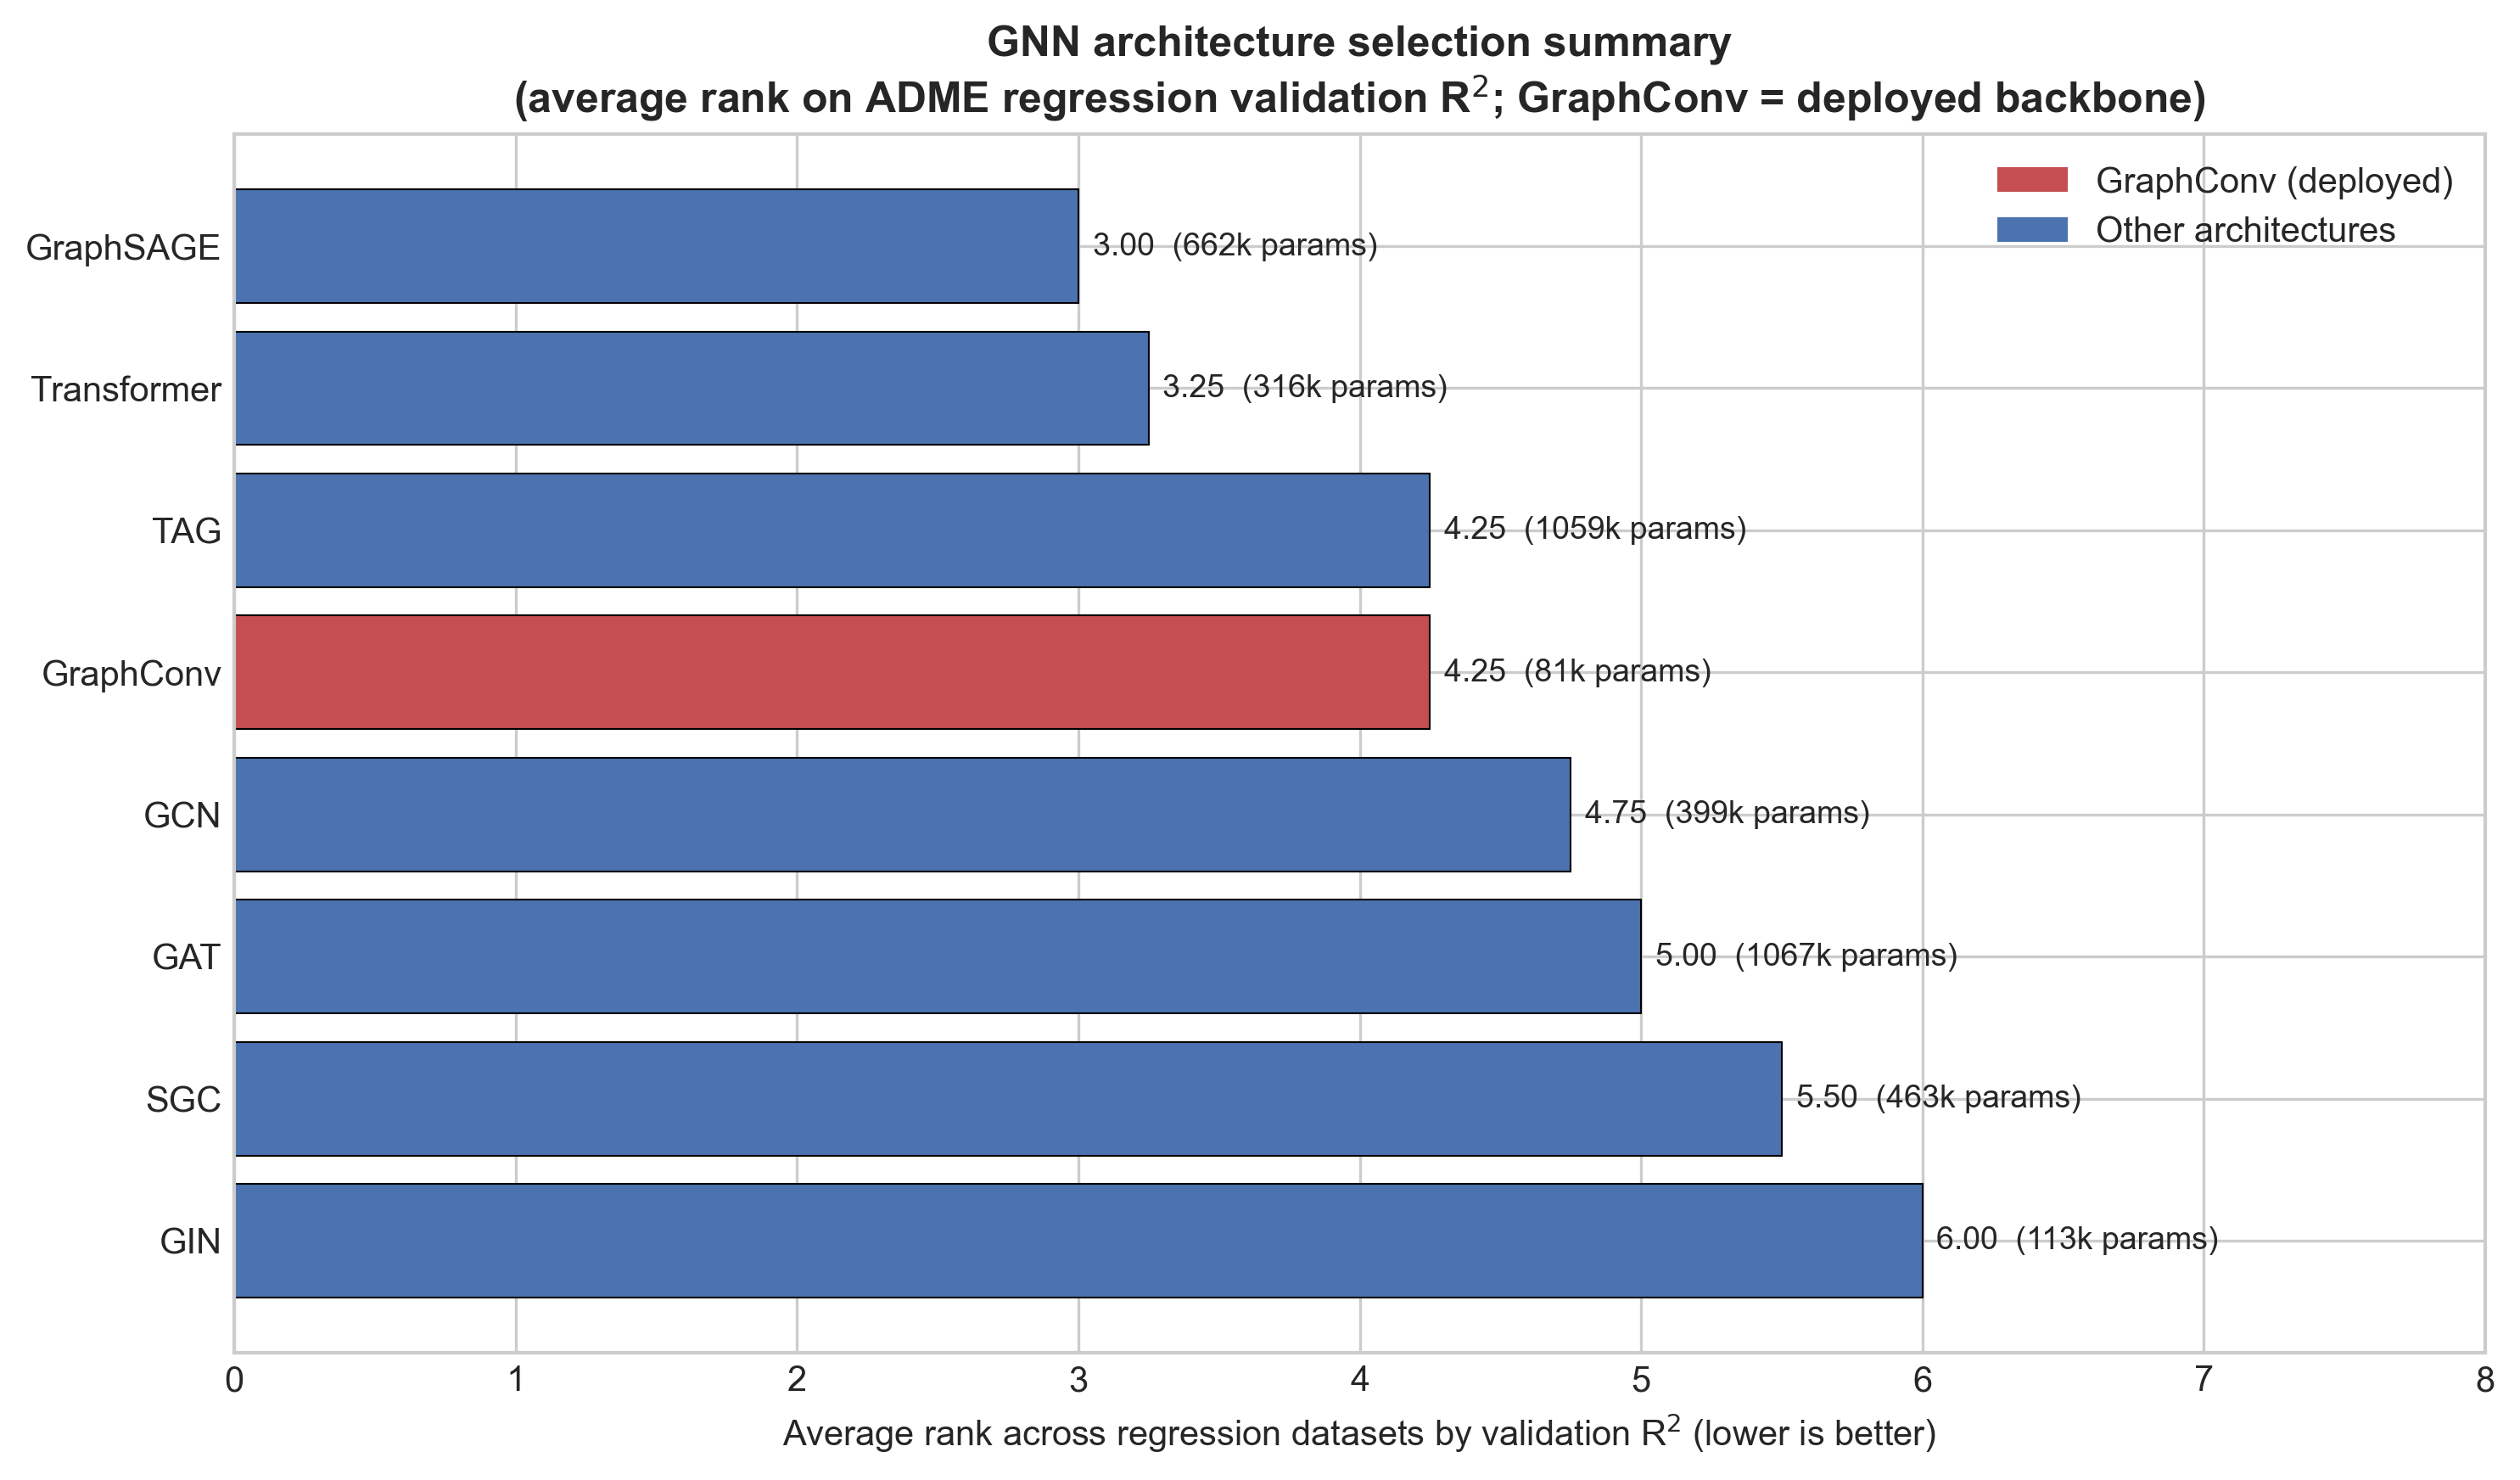
\includegraphics[width=0.95\textwidth,height=0.30\textheight,keepaspectratio]{arch_selection_summary.png}
    \caption{Preliminary architecture-selection summary showing average rank across the regression datasets by validation R$^2$ (lower is better); GraphConv (the deployed backbone) is highlighted. No architecture dominates and the per-dataset differences fall within the noise of these small datasets; GraphConv was adopted as a single representative backbone using validation metrics only.}
    \label{fig:arch_selection_summary}
\end{figure}

\begin{figure}[H]
    \centering
    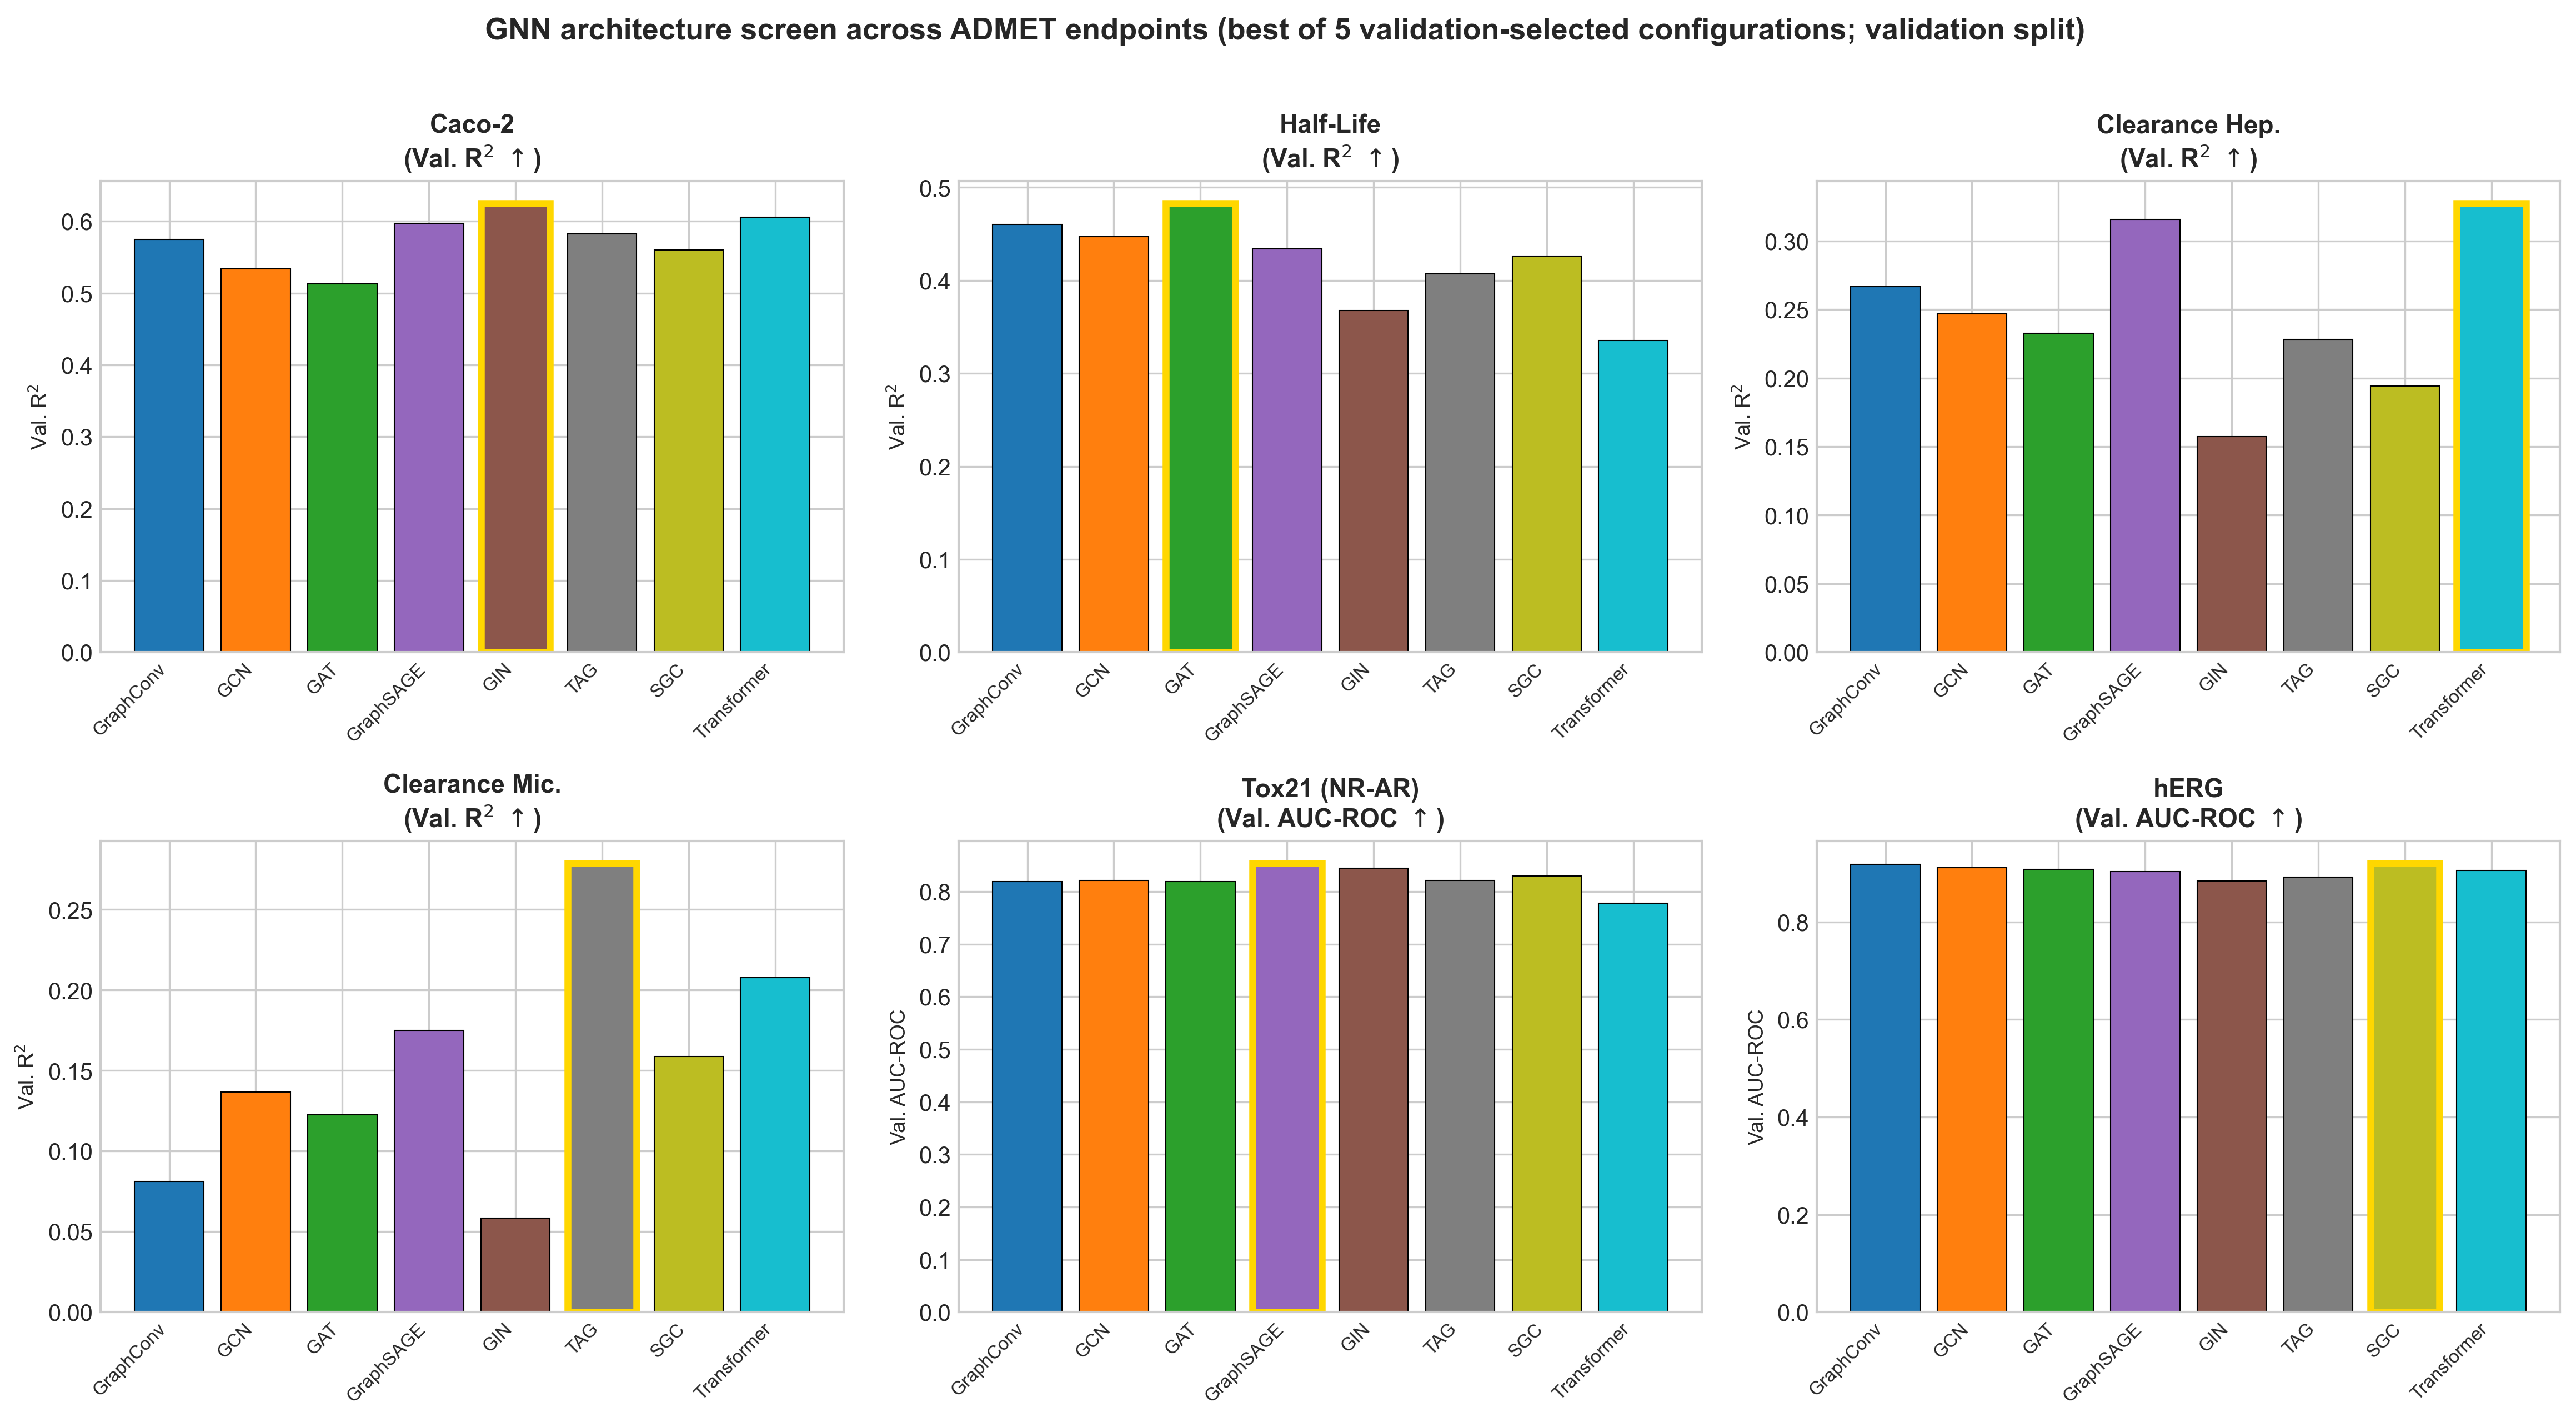
\includegraphics[width=0.95\textwidth,height=0.42\textheight,keepaspectratio]{arch_comparison_all_datasets.png}
    \caption{Per-dataset architecture comparison across all six benchmark endpoints (classification by validation AUC-ROC, regression by validation R$^2$; the selection basis). The weakly-learnable clearance and half-life endpoints are unstable across all eight architectures, whereas the structure-driven endpoints cluster within a narrow band.}
    \label{fig:arch_comparison}
\end{figure}

\section{Hyperparameter-Optimization Details}
\label{sec:supp_hpo}

\begin{table*}[!t]
\centering
\caption{HPO algorithms vs.\ Random Search (clean, leak-free re-run), each optimizer's \emph{validation-selected} configuration evaluated once on test across the $n=6$ datasets. Because the per-endpoint test metrics live on incomparable scales (R$^2$, occasionally pathologically negative, and AUC), we report direction-based and scale-controlled measures rather than a raw mean R$^2$/AUC difference. \textbf{W/T/L}: wins/ties/losses vs.\ Random Search. \textbf{Sign-test $p$}: exact two-sided binomial test on wins-vs-losses (ties dropped). \textbf{Norm.\ effect}: per-endpoint (optimizer$-$random) difference divided by the spread of all seven optimizers on that endpoint, averaged over the six endpoints (a scale-free, direction-normalized paired effect). \textbf{Sensitivity} columns recompute the mean paired difference with R$^2$ clipped to $[-1,1]$ and floored at $0$ (AUC untouched). All 95\% CIs are $10{,}000$-resample percentile bootstraps over the six paired differences. \emph{No optimizer is significant under the sign test, and every scale-free / clipped interval spans zero}; only the aggressively compressed floor-$0$ variant shows two marginal effects (ABC slightly $+$, SA slightly $-$), neither indicating a consistent winner. So none consistently outperforms Random Search under the 50-trial budget. Full per-trial histories are released with the code.}
\label{tab:best_results}
\small
\setlength{\tabcolsep}{4pt}
\begin{tabular}{lccccc}
\toprule
\textbf{Optimizer} & \textbf{W/T/L} & \textbf{Sign $p$} & \textbf{Norm.\ effect [95\% CI]} & \textbf{Clip $[-1,1]$ mean [95\% CI]} & \textbf{Floor-0 mean [95\% CI]} \\
\midrule
PSO & 2/0/4 & 0.69 & $-0.16$ [$-1.35$, $+1.25$] & $+0.174$ [$-0.084$, $+0.612$] & $+0.033$ [$-0.036$, $+0.124$] \\
ABC & 5/0/1 & 0.22 & $+0.52$ [$-0.45$, $+1.38$] & $+0.026$ [$-0.292$, $+0.311$] & $+0.032$ [$+0.000$, $+0.091$] \\
GA  & 3/0/3 & 1.00 & $+0.01$ [$-1.41$, $+1.40$] & $+0.169$ [$-0.067$, $+0.536$] & $+0.020$ [$-0.040$, $+0.086$] \\
SA  & 1/0/5 & 0.22 & $-0.77$ [$-1.82$, $+0.55$] & $-0.135$ [$-0.471$, $+0.171$] & $-0.018$ [$-0.031$, $-0.006$] \\
HC  & 3/0/3 & 1.00 & $+0.02$ [$-1.13$, $+1.37$] & $+0.034$ [$-0.440$, $+0.556$] & $+0.014$ [$-0.021$, $+0.062$] \\
TPE & 2/0/4 & 0.69 & $+0.01$ [$-1.02$, $+1.16$] & $+0.105$ [$-0.075$, $+0.329$] & $+0.027$ [$-0.024$, $+0.114$] \\
\bottomrule
\end{tabular}
\end{table*}

\begin{table}[H]
\centering
\caption{Hyperparameter search space for GNN models. The three MLP-head layer widths are sampled independently and then sorted in descending order (Layer~1~$\geq$~Layer~2~$\geq$~Layer~3) to yield a funnel-shaped prediction head.}
\label{tab:search_space}
\small
\begin{tabular}{ll}
\toprule
\textbf{Hyperparameter} & \textbf{Search Space} \\
\midrule
Hidden Dimensions & \{64, 96, 128, 192, 256, 384, 512\} \\
Number of Layers & \{3, 4, 5, 6, 7\} \\
Learning Rate & [1e-4, 1e-2] (log-uniform) \\
Weight Decay & [1e-6, 1e-2] (log-uniform) \\
MLP Head Layer 1 & \{128, 192, 256, 384, 512\} \\
MLP Head Layer 2 & \{64, 96, 128, 192, 256\} \\
MLP Head Layer 3 & \{32, 48, 64, 96, 128\} \\
\bottomrule
\end{tabular}
\end{table}

\begin{table*}[!t]
\centering
\caption{HPO-algorithm comparison (clean re-run): test performance of each optimizer's \emph{validation-selected} configuration across datasets (regression R$^2$, classification AUC-ROC). Shown for transparency; optimizers are compared statistically against Random Search in Table~\ref{tab:best_results}, and no optimizer is ever selected using test data. Regression R$^2$ is highly unstable on the weakly-learnable clearance endpoints, so per-optimizer regression values should not be over-interpreted.}
\label{tab:hpo_results}
\scriptsize
\begin{tabular}{lccccccc}
\toprule
\textbf{Dataset} & \textbf{PSO} & \textbf{ABC} & \textbf{GA} & \textbf{SA} & \textbf{HC} & \textbf{Random} & \textbf{TPE} \\
\midrule
\multicolumn{8}{l}{\emph{Regression (R$^2$ $\uparrow$)}} \\
\midrule
Caco2\_Wang & 0.508 & 0.553 & 0.450 & 0.519 & 0.519 & 0.552 & 0.515 \\
Half\_Life\_Obach & 0.119 & 0.211 & 0.193 & $-$0.285 & 0.037 & 0.035 & 0.274 \\
Clearance\_Hep. & $-$0.269 & $-$0.762 & $-$0.219 & $-$1.351 & $-$0.989 & $-$0.114 & $-$0.283 \\
Clearance\_Mic. & 0.235 & $-$0.387 & 0.058 & $-$0.529 & 0.130 & $-$3.288 & $-$0.365 \\
\midrule
\multicolumn{8}{l}{\emph{Classification (AUC-ROC $\uparrow$)}} \\
\midrule
Tox21 (NR-AR) & 0.739 & 0.757 & 0.730 & 0.739 & 0.758 & 0.743 & 0.726 \\
hERG & 0.738 & 0.810 & 0.830 & 0.771 & 0.777 & 0.810 & 0.787 \\
\bottomrule
\end{tabular}
\end{table*}

\begin{figure}[!t]
    \centering
    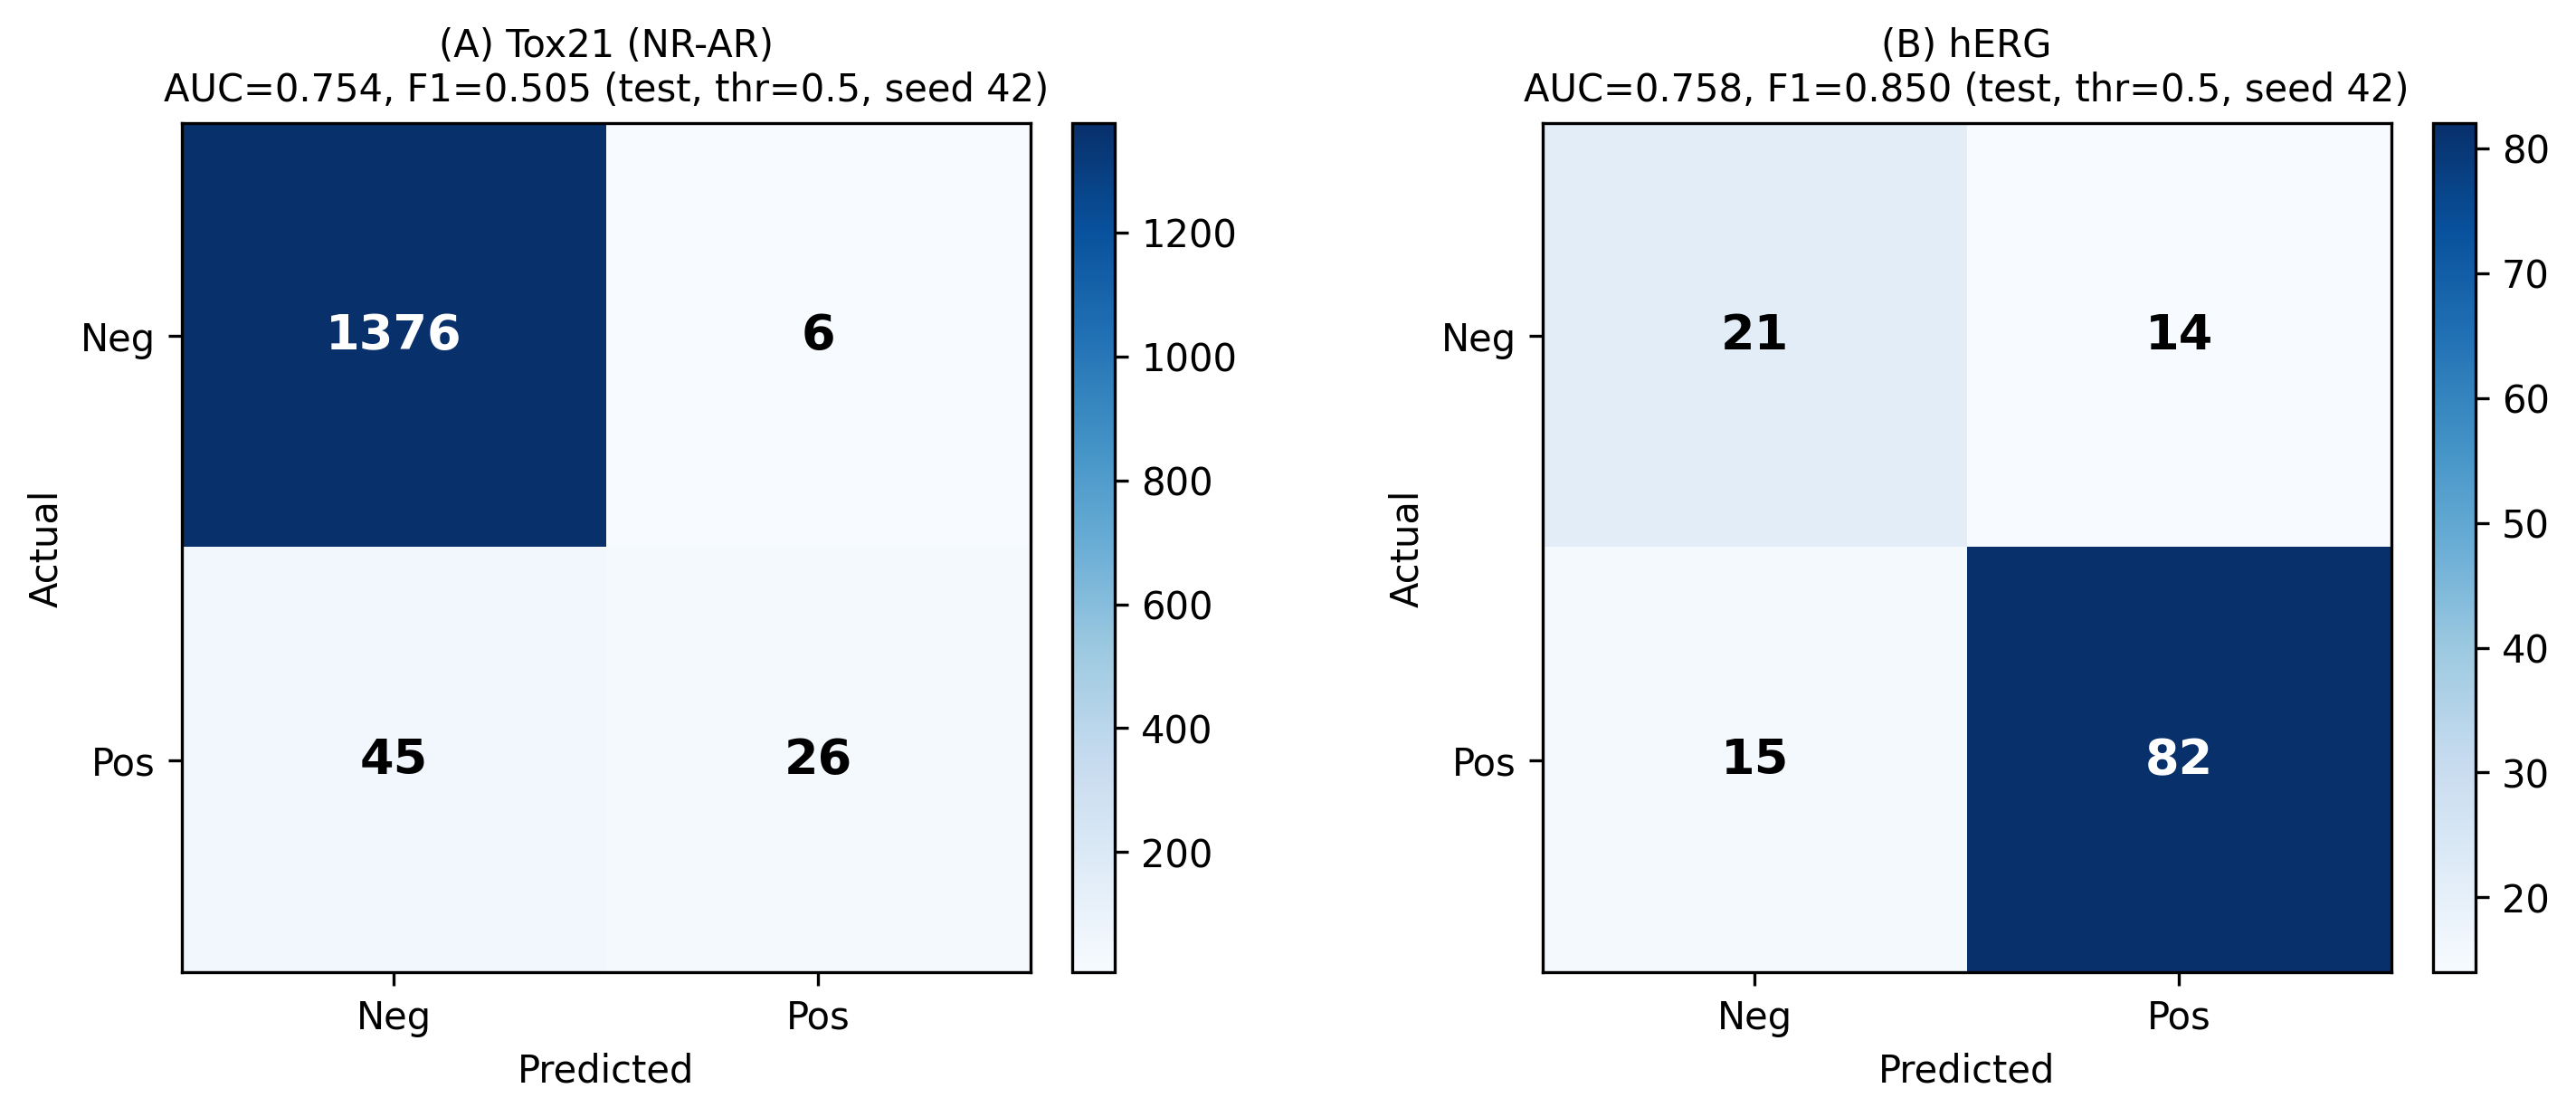
\includegraphics[width=\columnwidth,height=0.28\textheight,keepaspectratio]{confusion_matrices.png}
    \caption{Confusion matrices for the GNN's validation-selected configuration on the two toxicity tasks, on the held-out test set at the standard $0.5$ decision threshold (seed 42). (A) Tox21 shows majority-class bias due to extreme imbalance (F1 = 0.51). (B) hERG shows balanced performance (F1 = 0.85). Across-seed, threshold-tuned aggregates (mean over ten seeds) are reported in Fig.~\ref{fig:toxicity_stability} and the imbalance-metric text.}
    \label{fig:confusion_matrices}
\end{figure}

\begin{figure}[!t]
    \centering
    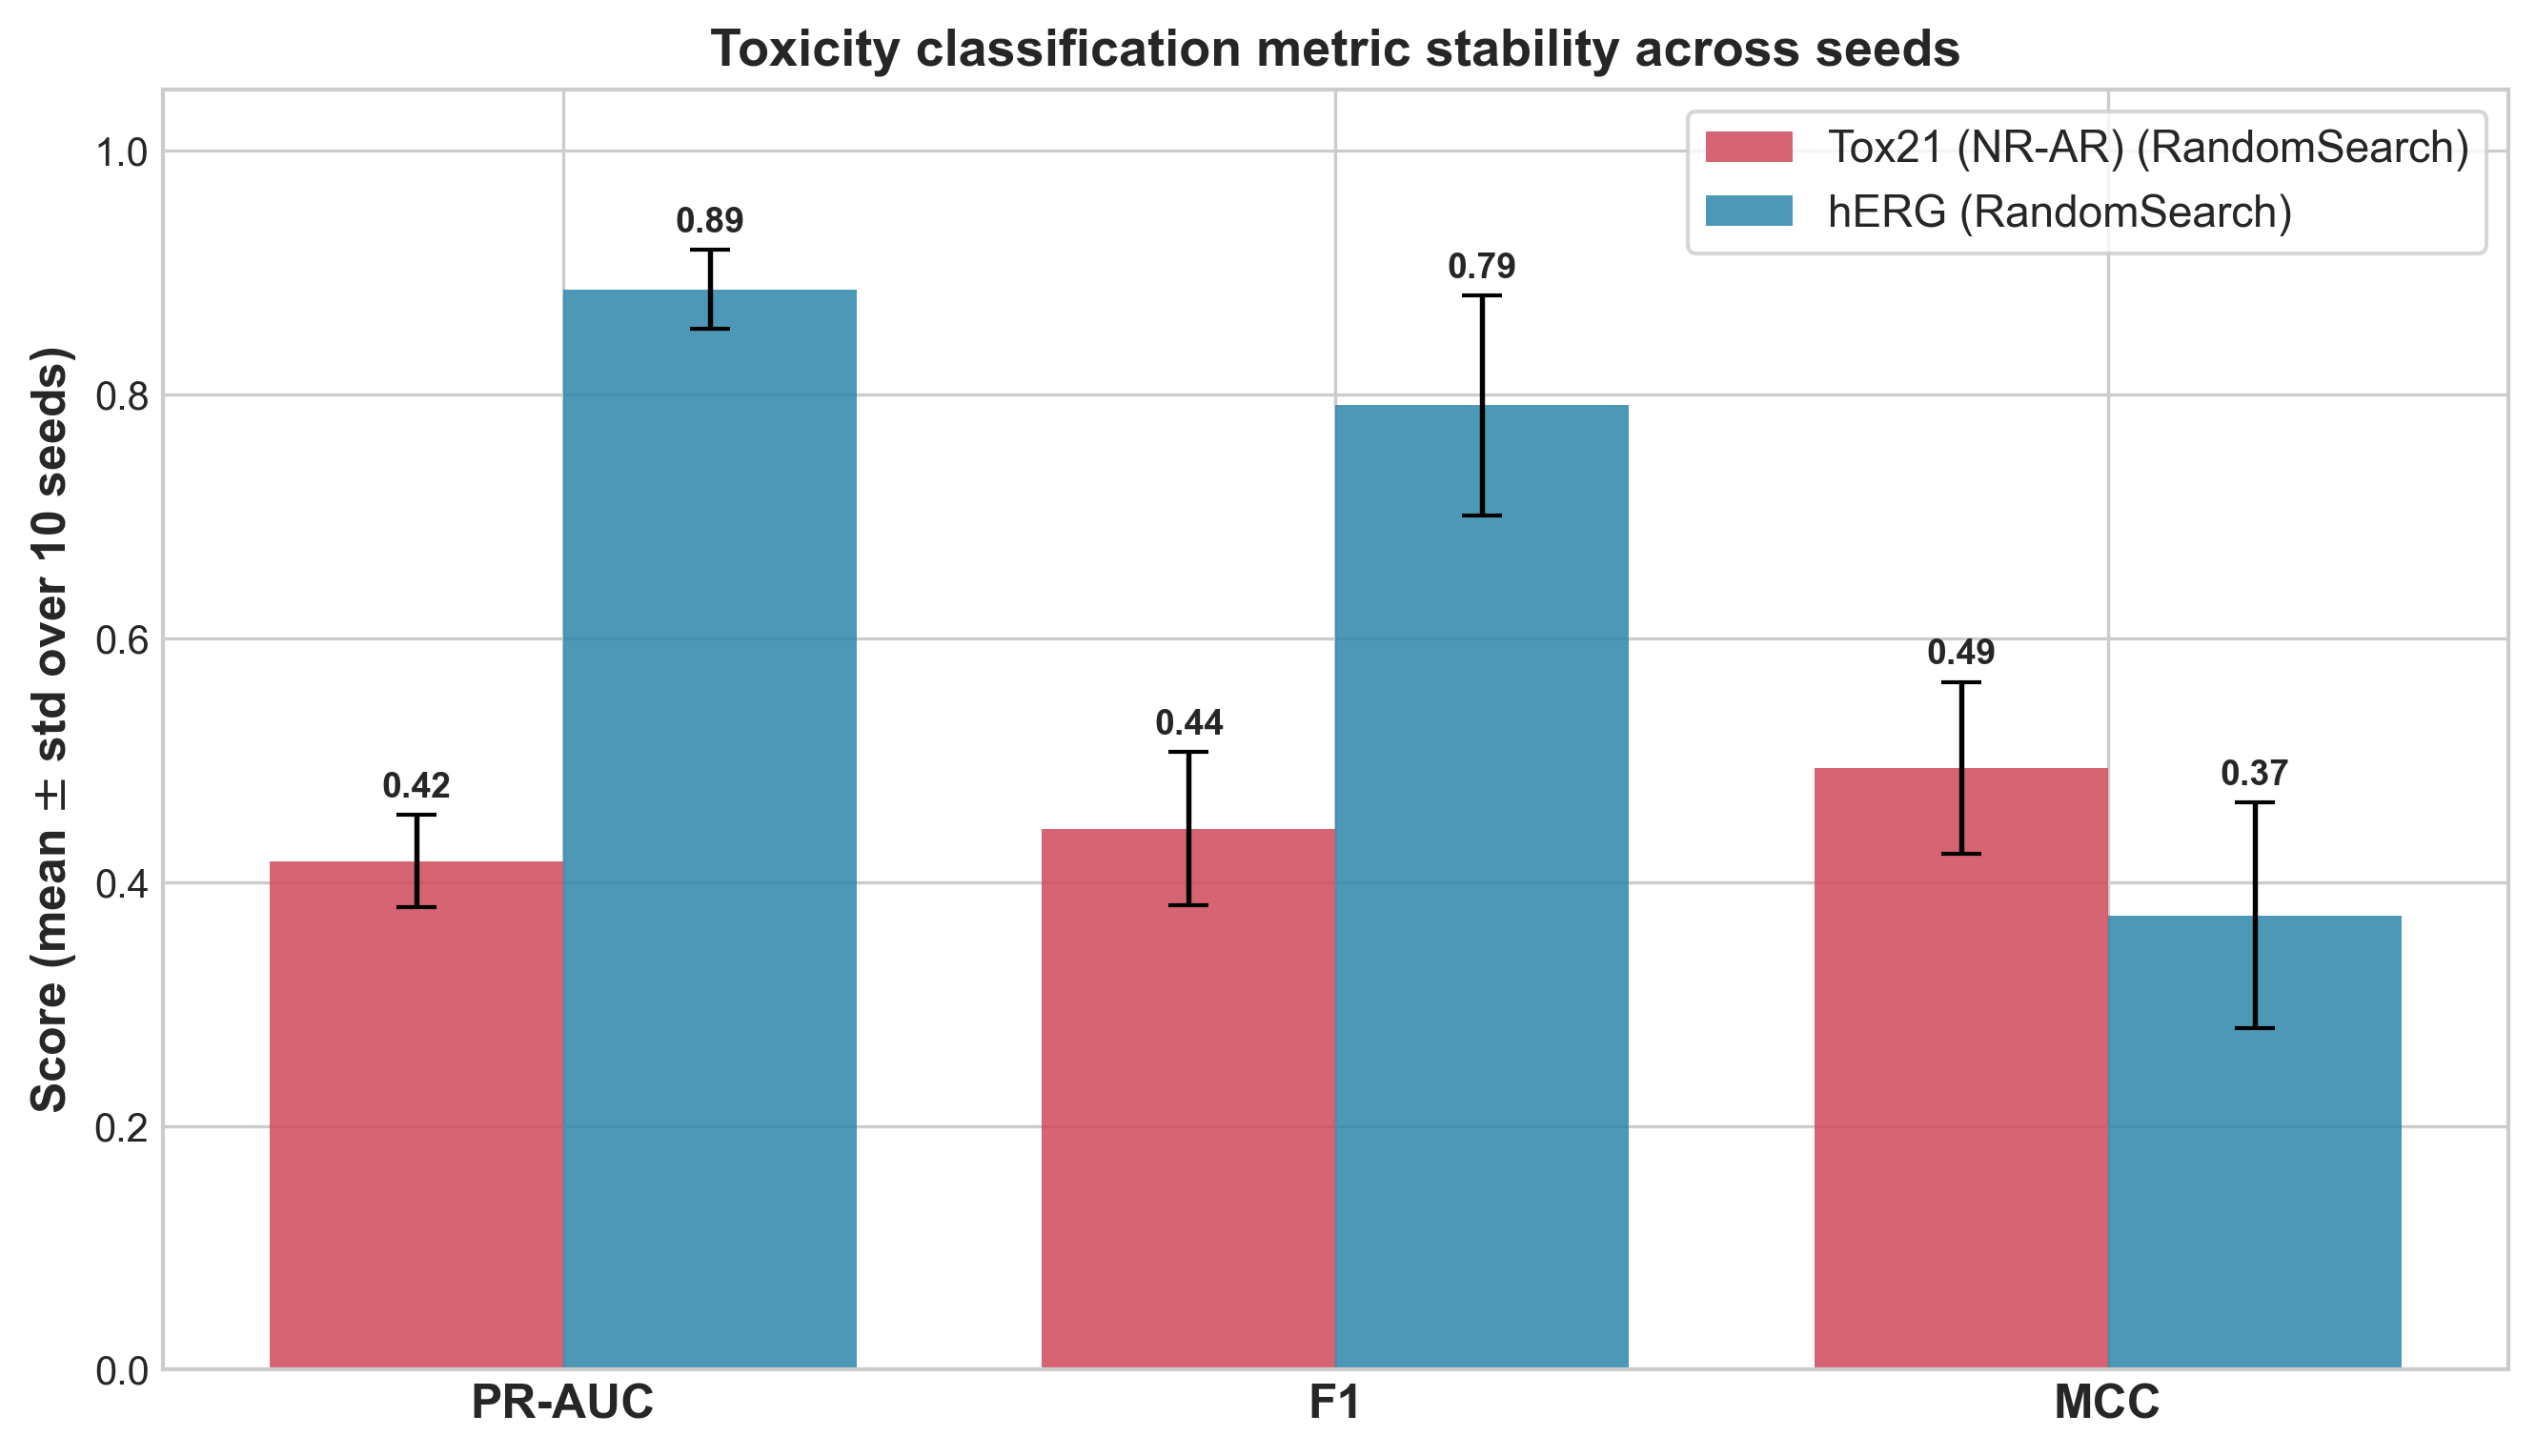
\includegraphics[width=\columnwidth,height=0.30\textheight,keepaspectratio]{toxicity_metric_stability.png}
    \caption{Across-seed stability of the imbalance-aware toxicity metrics (PR-AUC, F1, MCC). Bars show the mean over ten seeds and error bars show $\pm$ one standard deviation. These imbalance-aware summaries use mean $\pm$ standard deviation to quantify across-seed variability; the primary AUC-ROC results are summarized using median [min--max] in the main manuscript. Across-seed variability is modest for both endpoints, with the threshold-dependent F1 and MCC somewhat more variable on hERG than on Tox21.}
    \label{fig:toxicity_stability}
\end{figure}

\end{document}
